\begin{exercice*}
        Les figures 2 et 3 sont respectivement un agrandissement et une réduction de la figure 1.

        Terminer les construction. 

        %\hspace*{-15mm}
        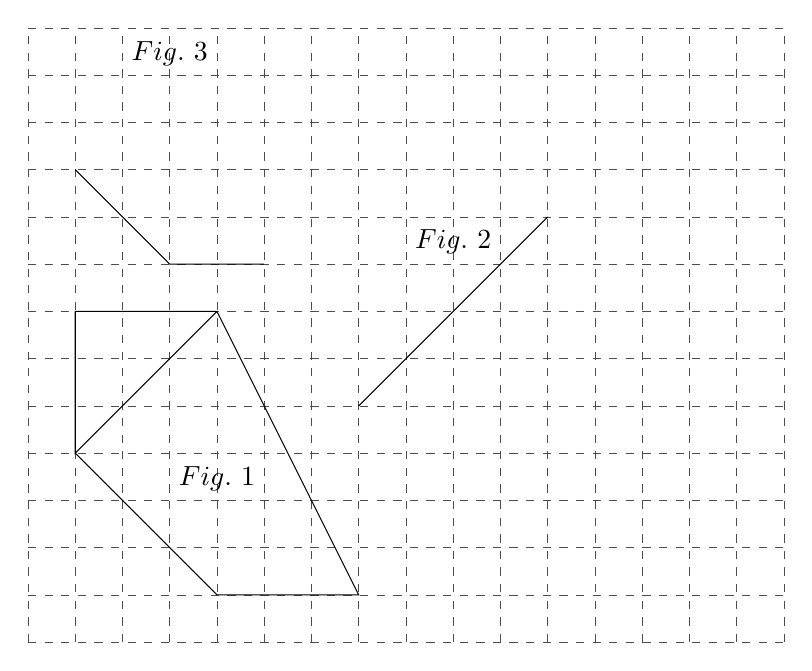
\begin{tikzpicture}[scale = 0.6]
                \draw[help lines, color=black!70, dashed] (0,0) grid (16,13);                
                \coordinate[label=above:$Fig.~1$] (F) at (4,3);        
                \coordinate (A) at (1,7);
                \coordinate (B) at (4,7);
                \coordinate (C) at (7,1);
                \coordinate (D) at (4,1);
                \coordinate (E) at (1,4);
                \draw (A)--(B)--(C)--(D)--(E)--(A)--(E)--(B);
                \coordinate[label=above:$Fig.~3$] (F1) at (3,12);        
                \coordinate (A1) at (1,12);
                \coordinate (B1) at (3,12);
                \coordinate (C1) at (5,8);
                \coordinate (D1) at (3,8);
                \coordinate (E1) at (1,10);
                \draw (C1)--(D1)--(E1);
                \coordinate[label=above:$Fig.~2$] (F2) at (9,8);        
                \coordinate (A2) at (7,9);
                \coordinate (B2) at (11,9);
                \coordinate (C2) at (15,1);
                \coordinate (D2) at (11,1);
                \coordinate (E2) at (7,5);
                \draw (E2)--(B2);
        \end{tikzpicture}

\end{exercice*}
\begin{corrige}
    %\setcounter{partie}{0} % Pour s'assurer que le compteur de \partie est à zéro dans les corrigés
    \phantom{rrr}  
    
    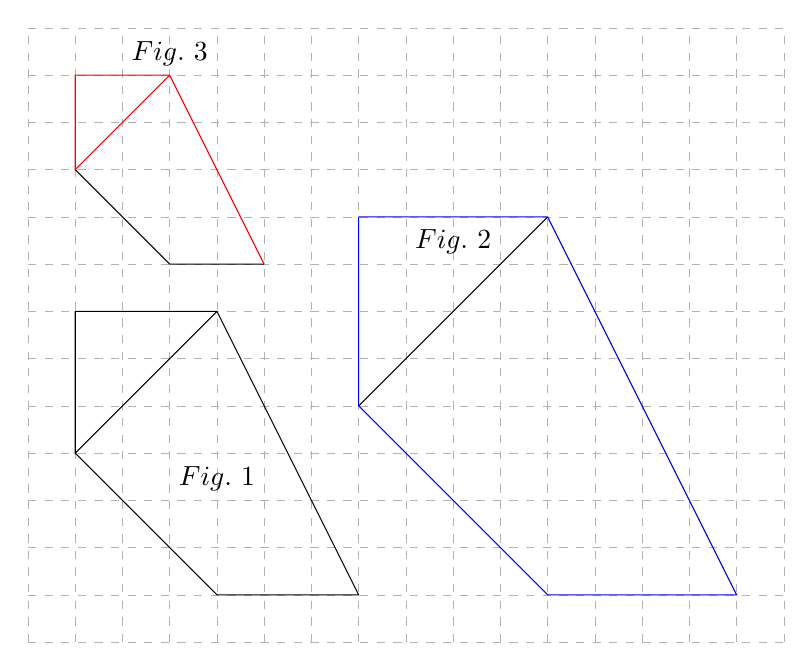
\begin{tikzpicture}[scale = 0.6]
        \draw[help lines, color=black!30, dashed] (0,0) grid (16,13);                
        \coordinate[label=above:$Fig.~1$] (F) at (4,3);        
        \coordinate (A) at (1,7);
        \coordinate (B) at (4,7);
        \coordinate (C) at (7,1);
        \coordinate (D) at (4,1);
        \coordinate (E) at (1,4);
        \draw (A)--(B)--(C)--(D)--(E)--(A)--(E)--(B);
        \coordinate[label=above:$Fig.~3$] (F1) at (3,12);        
        \coordinate (A1) at (1,12);
        \coordinate (B1) at (3,12);
        \coordinate (C1) at (5,8);
        \coordinate (D1) at (3,8);
        \coordinate (E1) at (1,10);
        \draw (C1)--(D1)--(E1);
        \draw[color=red] (A1)--(B1)--(C1);
        \draw[color=red] (E1)--(A1)--(E1)--(B1);
        \coordinate[label=above:$Fig.~2$] (F2) at (9,8);        
        \coordinate (A2) at (7,9);
        \coordinate (B2) at (11,9);
        \coordinate (C2) at (15,1);
        \coordinate (D2) at (11,1);
        \coordinate (E2) at (7,5);
        \draw (E2)--(B2);
        \draw[color=blue] (A2)--(B2)--(C2)--(D2)--(E2)--(A2);        
    \end{tikzpicture}     
\end{corrige}

